% Indicate the main file. Must go at the beginning of the file.
% !TEX root = ../main.tex

%%%%%%%%%%%%%%%%%%%%%%%%%%%%%%%%%%%%%%%%%%%%%%%%%%%%%%%%%%%%%%%%%%%%%%%%%%%%%%%%
% 03_methods
%%%%%%%%%%%%%%%%%%%%%%%%%%%%%%%%%%%%%%%%%%%%%%%%%%%%%%%%%%%%%%%%%%%%%%%%%%%%%%%%

\section{Methods}
\label{methods}

    \subsection{Dataset}

    As part of the Wildlife@Campus project, a labeled dataset was created to train a deep learning algorithm.
    This dataset is divided into seven sessions -- indicating the project stage where the data was added to the dataset.
    The images are grouped into sequences, each sequence representing a sightin of an animal.
    Somehow the sequences are not standardized in length and range from 1 to 915 images per sequence.
    It is worth noting that in future use cases, the sequence length will likely be more standardized.
    The actual length will depend on the camera settings -- common settings such as 1, 3, 5, or 10 images per trigger -- which can be extracted from the EXIF information of the images.
    For this project, the sequences will be used as they are, and the length will not be standardized.
    The dataset provides two types of labels: the first one is not yet standardized troughout the sessions and contains a variety of labels for the same species.
    For example scientific names and common names are used interchangeably, and there are different spellings.
    The second type is a simplified and standardized version with some visually not distinguishable species grouped together.
    For this project, only the simplified labels will be used.
    To get an overview of the available sequences per label, refere to \autoref{fig:sequenceperlabel}.
    The category \texttt{other} represents sequences containing more than one species, this is a result of the process creating the sequences.
    Furthermore the category \texttt{NaN} represents sequences not labeled -- both will be excluded from the from the dataset.
    The category \texttt{glis\_glis} is represented in only four sequences, which is simply not enough to actually train the model to detect it.
    For this reason, it will be excluded from the dataset as well.
    This leaves four categories for the classification task: \texttt{apodemus\_sp}, \texttt{cricetidae}, \texttt{soricidae}, and \texttt{mustela\_erminea}.

    \begin{figure}[ht]
    \centering
    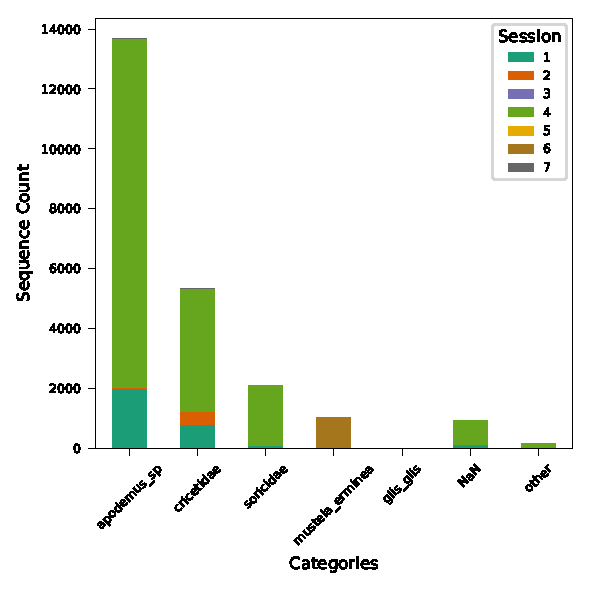
\includegraphics{figures/label2_session.pdf}
    \caption{Available sequences per label colored by session.}
    \label{fig:sequenceperlabel}
    \end{figure}

    \subsection{Processing}

    The processing of the images is divided into two main steps: 
    In a first step a detector is applied to identify the regions of interest (ROI) for the images, and to select which images are actually used for training.
    In a second step, the ROIs are processed to be feed into the model.

        \subsubsection{Detection and Selection}
        
        In this project, the Megadetector (MD) \autocite{morrisEfficientPipelineCamera2025} is used to identify regions of interest (ROI) on all the images.
        The MD outputs a list of bounding boxe (BBox) for detected objects labeled \textit{animal}, \textit{human} or \textit{vehicle} with a corresponding confidence value.
        For each image only the BBox with the highest confidence score -- above a threshold of 0.5 -- for the label \textit{animal} is considered.
        The percentage of images discarded dew to this process is  shown per sequence in \autoref{fig:lost_images}.
        An example of how this detections look like is shown in \autoref{fig:detection_example}.

        \begin{figure}[ht]
        \centering
        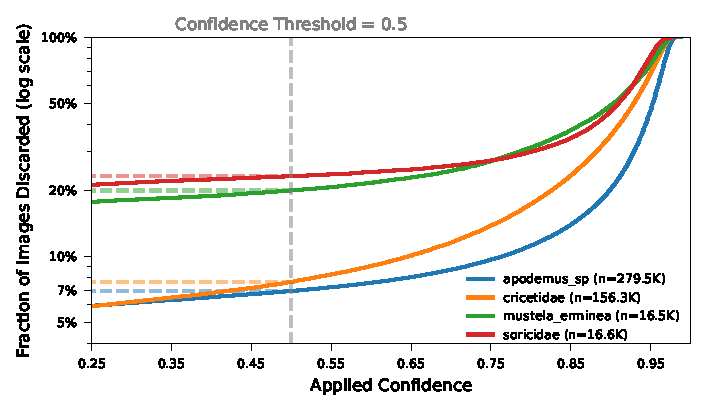
\includegraphics{figures/discarded_img_by_conf.pdf}
        \caption{Fraction of images discarded per category for a detection confidence threshold of 0.5.}
        \label{fig:lost_images}
        \end{figure}

        \begin{figure}[ht]
        \centering
        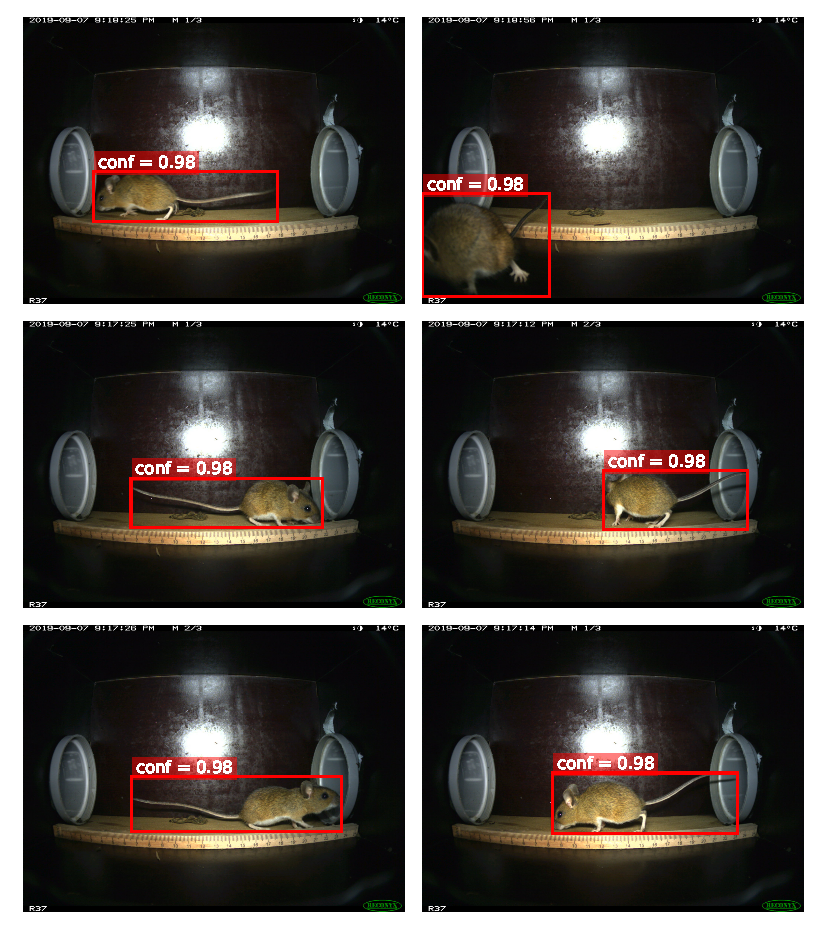
\includegraphics{figures/detections_on_a_sequence.pdf}
        \caption{Example of how the detections look like. The bounding boxes are the highest confidence detections for the sequence 1001824 a sample from the \textit{apodemus\_sp} category.}
        \label{fig:detection_example}
        \end{figure}

        \subsubsection{Image Preprocessing}
        To process the images a custom transformation pipline was implemented using transform version 2 from the torchvision library and a custom crop function.
        This transformation is applied on the fly by the PyTorch DataLoader.
        Cropping was done using the BBoxes from the MD detection extending the BBox in order to cut the ratio expected by the model applied.
        In the case that the extended BBox surpasses the image border the image is padded with black pixels.
        After cropping the image is resized to the expected input size of the model.
        The images are then converted to a tensor and normalized using the mean and standard deviation calculated on the dataset itself.
        To calculate mean and standard deviation the whole dataset was used since it is quite resource intensive to calculate and the same values are used for all folds.
        To create the most accurate mean and standard deviation for the actual model input only the best BBox area per image is used.
        Data augmentation a well established way to improve model's generalization \autocite{shortenSurveyImageData2019} was implemented and considered as an option but not actually used in the end.

    \subsection{Data Splitting}

    The dataset is split into five folds using a stratified split based on the classes.
    A custom helper function was implemented to ensure the splits are done on a sequence level, meaning no sequence is ever split between folds, while still maintaining a balanced distribution of images across the folds.
    For each class in the dataset, all the sequences are shuffled using a fixed seed for reproducibility resulting in two lists: one with the sequence ids and one with the corresponding sequence lengths.
    To build five stratified folds, it steps through the shuffled list of sequence-lengths and chooses cut-points so that each fold's sum of images is as close as possible to one-fifth of that class's total images.
    In this way, every fold ends up with roughly the same number of images per class, and no sequence is ever split between folds.

    \subsection{Model}
    - how the models where adapted for the task (tool to detect type of last layer and rebuild it to fit the num classes)

    - description of the used models

    \subsection{Training}

    The training was implemented using the PyTorch Lightning framework \autocite{falconPyTorchLightning2025}.
    The training process is divided into four main steps:
    \begin{enumerate}
        \item Loading the dataset and applying the preprocessing steps described above.
        \item Initializing the model with the appropriate architecture and the number of classes.
        \item Training the model using the training set and validating it using the validation set.
        \item Testing the model on the test set to evaluate its performance.
    \end{enumerate}

    - description of the training using the PyTorch Lightning framework 

    - used parameters

    \subsection{Sequence Classification}
    - how the selection on a sequence level is derived from the image level classification

    - could possibly be included under evaluation

    \subsection{Evaluation}
    - description of the used metrics to describe the model performance

    - question to clarify: what is this balanced accuracy actually?
